\documentclass{scrartcl}
\usepackage[utf8]{inputenc}
\usepackage{bussproofs}
\usepackage{scrpage2}
\usepackage{rotating}
\usepackage{listings}
\usepackage{amsmath}
\usepackage{amsfonts}
%\usepackage{mathtools}
\usepackage{hyperref}
\pagestyle{scrheadings}
\renewcommand{\thesubsection}{\alph{subsection}}
\clearscrheadfoot
\ohead[]{Nikolas Zeitler, Joshua Hartmann, Alexander Diegel}
\cfoot[\pagemark]{\pagemark}
\author{Nikolas Zeitler, Joshua Hartmann, Alexander Diegel}
\title{Maschinelles Lernen Blatt 3}

%INFO bitte mit TODO-tags arbeiten, dann sieht man es im Studio auf der linken seite
%TODO Beispiel 

\begin{document}
\maketitle
\section{Fragen zur Vorlesung}
\subsection*{a) Darstellung als log-likelihood und warum sinnvoll?}
\[ ln (p(D|\vartheta)) = \Sigma^n_{k=1} ln (p(D|\vartheta)) \]
Sinnvoll: \\
%wikipedia:
Kann im Rahmen der Maximum-Likelihood-Methode verwendet werden. Dies ist ein parametrisches Schätzverfahren. Dabei wird der Parameter als Schätzung gewählt, der abhängig von der Verteilung die Daten am besten erklärt.\\
Der Logarithmus wandelt den Produktterm in einen Summenterm um. Eine Summe ist idR. einfacher zu maximieren 
als ein Produkt (Rechenoperationen gehen schneller aus Computersicht) da jeder Term für sich abgeleitet werden kann und keine Produktregel angewandt werden muss.

Das Maximum des Ausdrucks bleibt auch weiterhin das Maximum des logarithmierten Ausdrucks, daher ist die Form dem Vorhaben nicht abträglich. 

Maximum Likelihood such Parameter, die die Trainingsdaten am besten erklären.
\subsection*{b) Wie berechnet man Erwartungswert und Standardabweichung}
Foliensatz 3 S.9 \\
%Mu/Sigma mit dächlein ? Tech befehl suchen
\[\mu = \frac{1}{n}\Sigma^n_{k=1}x_k \]

\[\sigma^2 = \frac{1}{n-1}\Sigma^n_{k=1}(x_k-\mu)^2 \]

\subsection*{c)Was ist die Hauptannahme bei der Bayesschen Parameterschätzung}
Da Bayes genutzt wird müssen die Messungen unabhängig sein. %TODO echt, wir hatten doch auch Multivariate? 
Die klassenabhängige Dichte $p(x|w_i,D)$ sei nur von den Daten der jeweiligen Klasse abhängig, und betrachten daher nur eine Klasse. Das $w_i$ entfällt also.
\subsection*{d)}
Um die Unsicherheit auszugleichen die wir mit dem geschätzten $\mu$ gemacht haben wird die bekannte Varianz um $\sigma_m^2$ vergößert. Deswegen gilt die Formel wie sie da steht.


\subsection*{e) Welche Fehler bei Parameterschätzung möglich}
Bei einer sehr hohen Standardabweichung braucht man entsprechend viele Messungen sonst ist das Ergebnis "geraten" und damit womöglich Fehlerhaft.\\
\begin{itemize}
	\item Bayes Fehler
	\item Modell- Fehler
	\item Schätzfehler
\end{itemize}
\subsection*{f) Unterschied Schätzfehler und Modellfehler}
Wikipedia: \\
Ein Modellfehler ergibt sich aus einem fehlerhaften Modellansatz. Solch ein Fehler ist kein statistisches Phänomen, sondern ein sog. Wirklichkeitsphänomen, kann also beispielsweise durch eine Korrektur der Modellstruktur behoben werden. \\
In der Statistik bezeichnet der Schätzfehler die Abweichung einer Schätzfunktion $\hat{\vartheta}$ vom unbekannten Parameter der Grundgesamtheit $\vartheta$. Er ist ein Maß für die Güte der Schätzfunktion (oder Interpolation). \\

Ein Modellfehler hat also nichts mit einem Statistischen Ergebnis zu tun.(Schätzfehler zu) Ein Modellfehler ist der Fehler den man hat wenn man von Grund auf von einem Fehlerhaften Modell ausgeht. \\

Der Schätzfehler verbessert sich mit zunehmender Anzahl an Stichproben, der Modellfehler bleibt.

\section{Maximum-Likelihood-Schätzung}
\subsection*{Nachweis, dass der Maximum-Likelihood-Schätzer für den Parameter $\mu$ dem Durchschnitt der Stichprobe entspricht. (10 Punkte)}
Es ist:\\
$p(x)=\frac{1}{(\sqrt{2\pi \sigma^2})} \cdot \exp(-\frac{(x_i-\mu)^2}{2\sigma^2})$\\
Da $\sigma$ bekannt ist und als Konstante betrachtet werden kann gilt für MLE:\\
$MLE: p(X|\mu)=\prod_{i=1}^{n}p(x_i) $\\
$=\prod_{i=1}^{n}\frac{1}{\sqrt{2\pi \sigma^2}} \cdot \exp(-\frac{(x_i-\mu)^2}{2\sigma^2}) $\\
$= \frac{1}{(2\pi \sigma)^{n/2}} \cdot \exp(-\frac{1}{2\sigma^2} \cdot \sum_{i=1}^{n}(x_i-\mu)^2)$\\\\
Mit Log-MLE:\\
$\ln(p(X|\mu))= -\frac{n}{2} \cdot \ln(2\pi \sigma) - \frac{1}{2\sigma^2} \cdot \sum_{i=1}^{n}(x_i-\mu)^2$\\\\
Ableiten nach $\mu$ ergibt:\\
$\frac{\partial p(X|\mu)}{\partial \mu} = \frac{1}{\sigma^2} \cdot \sum_{i=1}^{n}(x_i-\mu)$\\\\
Ableitung = 0 gdw. Summenterm 0 ergibt!\\
$\sum_{i=1}^{n}(x_i-\mu) = 0$\\
$\sum_{i=1}^{n}(x_i)-n \cdot \mu = 0$\\
$\mu = \frac{\sum_{i=1}^{n}x_i}{n}$

Damit ist gezeigt, dass der Schätzer von MLE für $\mu$ dem Durchschnitt der Stichprobe entspricht.
 

\section{Bayessche Parameterschätzung}
\subsection*{a) Paramterbeschreibung}
\begin{itemize}
	\item $\hat{\mu_n}$:\\
	Mittelwert der Stichprobe für n=0 wird er unendlich groß da er gemäß $\sum(x_i) /n$ berechnet wird. Für großes n nähert sich der Stichprobenmittelwert dem wahren Mittelwert der Verteilung immer mehr an. Für n = $\infty$ entspricht er dem wahren Mittelwert. Für kleines n ist der Mittelwert der Stichprobe gegenüber dem wahren Mittelwert der Verteilung mit Unsicherheit behaftet.
	\item $\mu_0$:\\
	A priori Schätzer für den Mittelwert. Ändert sich nicht für unterschiedliches n. 
	%TODO stimmt das mit \mu_0 so?
	\item $\sigma^2_0$:\\
	Gibt Unsicherheit für das geschätzte a priori $\mu_0$ an. Unabhängig von n.
	%TODO stimmt das mit \sigma^2_0 so?
	\item $\sigma^2$:\\
	Wahre Varianz der normalverteilten Zufallsvariablen. An der wahren Varianz ändert sich durch die Stichprobengröße ebenfalls nichts.
\end{itemize}

\subsection*{b) Auskunft $\sigma^2_n$}
$\sigma^2_n$ gibt die Unsicherheit für den, mit der Bayesschätzung, geschätzten Mittelwert $\mu_n$ nach n Samples an. Umso mehr Samples verwendet werden, desto kleiner wird die Varianz und desto mehr entspricht sie der wahren Varianz der Verteilung.


\subsection*{e) Plottet für jedes i die zu approximierende Funktion N(3,1) und die Bayessche Schätzung. Bayes ist rote Kurve}
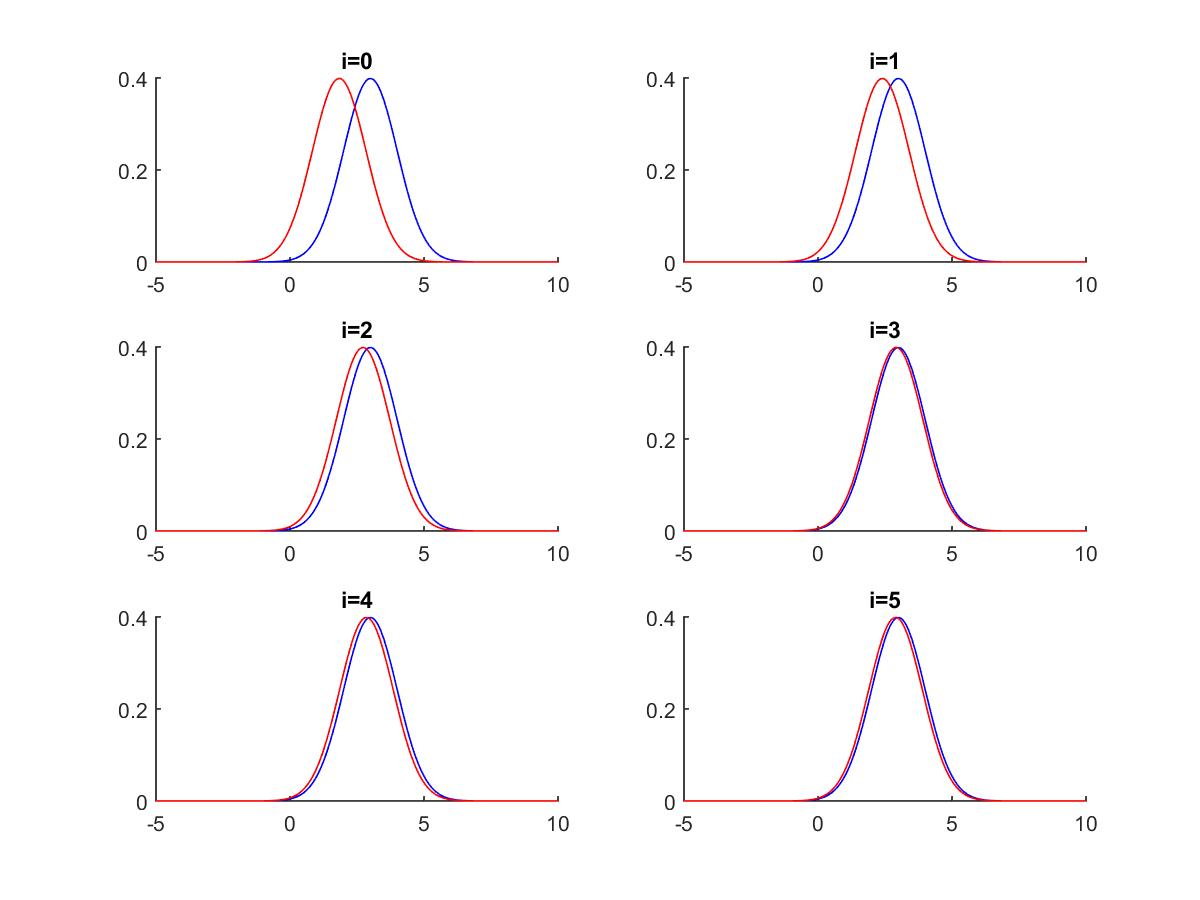
\includegraphics[width=1\textwidth]{plots/ApproxVsBayes.jpg} 

\subsection*{f)Angabe des quadratischen Fehlers }
%TODO TEAM: Ich bin vom Mean Square Error ausgegangen. Kann sein, dass was anderes gefragt war
\begin{itemize}
	\item i=0: 0.0108
	\item i=1: 0.0032
	\item i=2: 7.0277e-04
	\item i=3: 6.7479e-05
	\item i=4: 2.0726e-04
	\item i=5: 1.0817e-04
\end{itemize}

\subsection*{g) Beschreibt in eigenen Worten, wie sich Bayes im Vergleich zu Maximum-Likelihood verhält}
Bayes: Liefert Wahrscheinlichkeit für die geschätzten Parameter.\\
ML: Sucht Parameter, die Trainingsdaten am besten repräsentieren.

\end{document}
